\documentclass[./main_en.tex]{subfiles}
\graphicspath{{\subfix{./figs}}}

% ------------ main document ------------
\begin{document}
\nolinenumbers

% style setup
\newpage
\renewcommand{\headrulewidth}{0pt}
\thispagestyle{fancy}
%... then configure it
\fancyhf{} % Clear all header and footer fields.
\fancyfoot{} % clear all footer fields
\fancyfoot[C]{\thepage}

\par \hfill
\vspace{40mm}
\begin{adjustwidth}{45pt}{45pt}
\begin{center}
    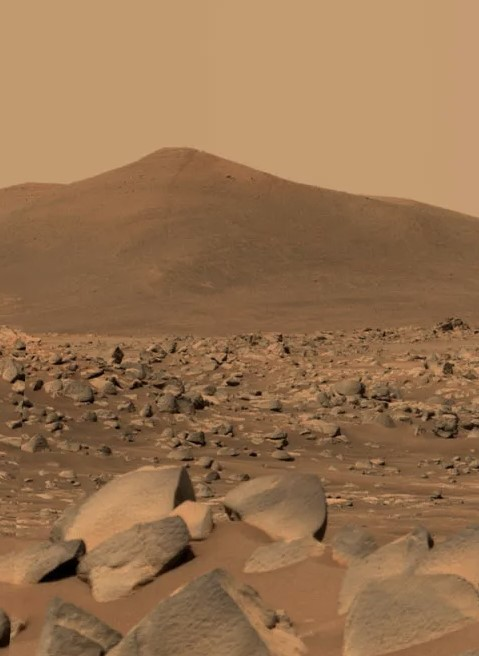
\includegraphics[scale=0.7]{figs/mars.jpg}\\
\end{center}
\vspace{10mm}
\noindent \textsf{Mars has a rocky and sandy terrain. Its atmosphere is composed of approximately 95\% carbon dioxide, with an average atmospheric pressure of about 600 Pa. Temperatures vary drastically, with average values around -60°C. The planet has no bodies of liquid water, and its surface is constantly exposed to cosmic and solar radiation due to the lack of a magnetic field.}
\end{adjustwidth}
\clearpage
\end{document}